\chapter{Supermarkt im Energieversorgungsnetz}
\label{chap:SEVN}
\minitoc

In diesem Kapitel wird anhand eines vier Knoten Beispielnetzes vorgestellt, Lösung Problem\todo{Der Einführungsabsatz ist zu
schreiben.}. Unabhängig von dem mathematischen Modell des Modellsupermarktes wird die Umsetzung der Implementierung
vorgestellt\todo{Was ist los?}.



\section{Anwendung der OOP am Modell}
In der \cref{vkb} wird ein einfaches vier Knoten Energieversorgungsnetz dargestellt. Am Knoten eins ist eine regenerative
elektrische Energiequelle, in diesem Fall ein Windpark, angeschlossen. Weitere konventionelle elektrische Energiequellen
befinden sich an den Knoten zwei und drei. Die passiven Lasten befinden sich am Knoten zwei und vier. Der Kältespeicher ist am
Knoten zwei angeschlossen. Die Knoten sind untereinander durch Leitungen verbunden, durch die elektrische Energie in
bestimmter Menge und in bestimmte Richtungen fließen.

\begin{figure}[h]
\caption{Vier Knoten Beispiel}
	\label{vkb}
	\begin{center}
	\includegraphics[scale=0.3]{images/SEVN/SEVN}
	\end{center}
\end{figure}

Für die 

\begin{figure}[h]
\caption{Klassendiagramm Modellkonstrukt}
	\label{klassendiagramm}
	\begin{center}
	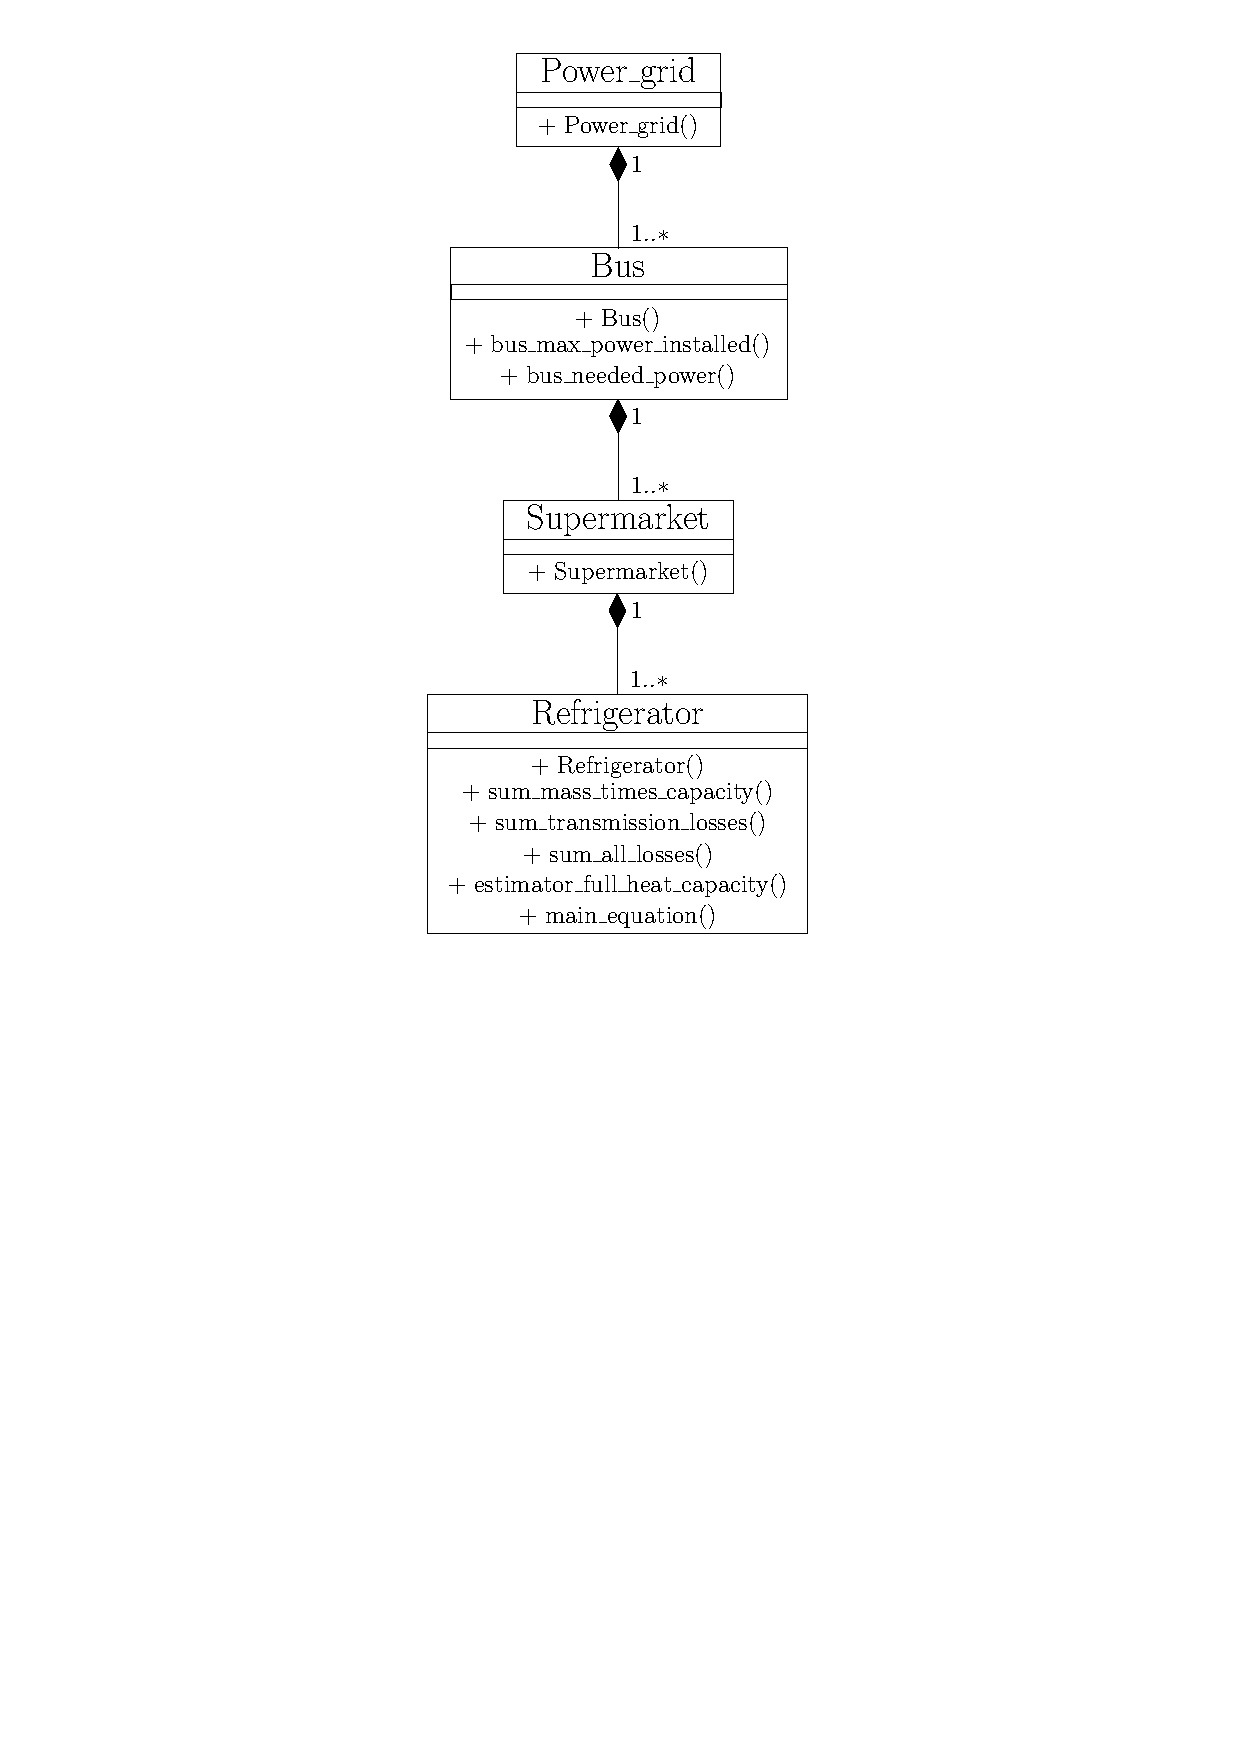
\includegraphics[scale=0.8]{images/Theorie_Super/class_diagramm}
	\end{center}
\end{figure}

Hier noch ein Zwischentext.

\begin{figure}[h]
\caption{Sequenzdiagramm Modellkonstrukt}
	\label{uml_sequence}
	\begin{center}
	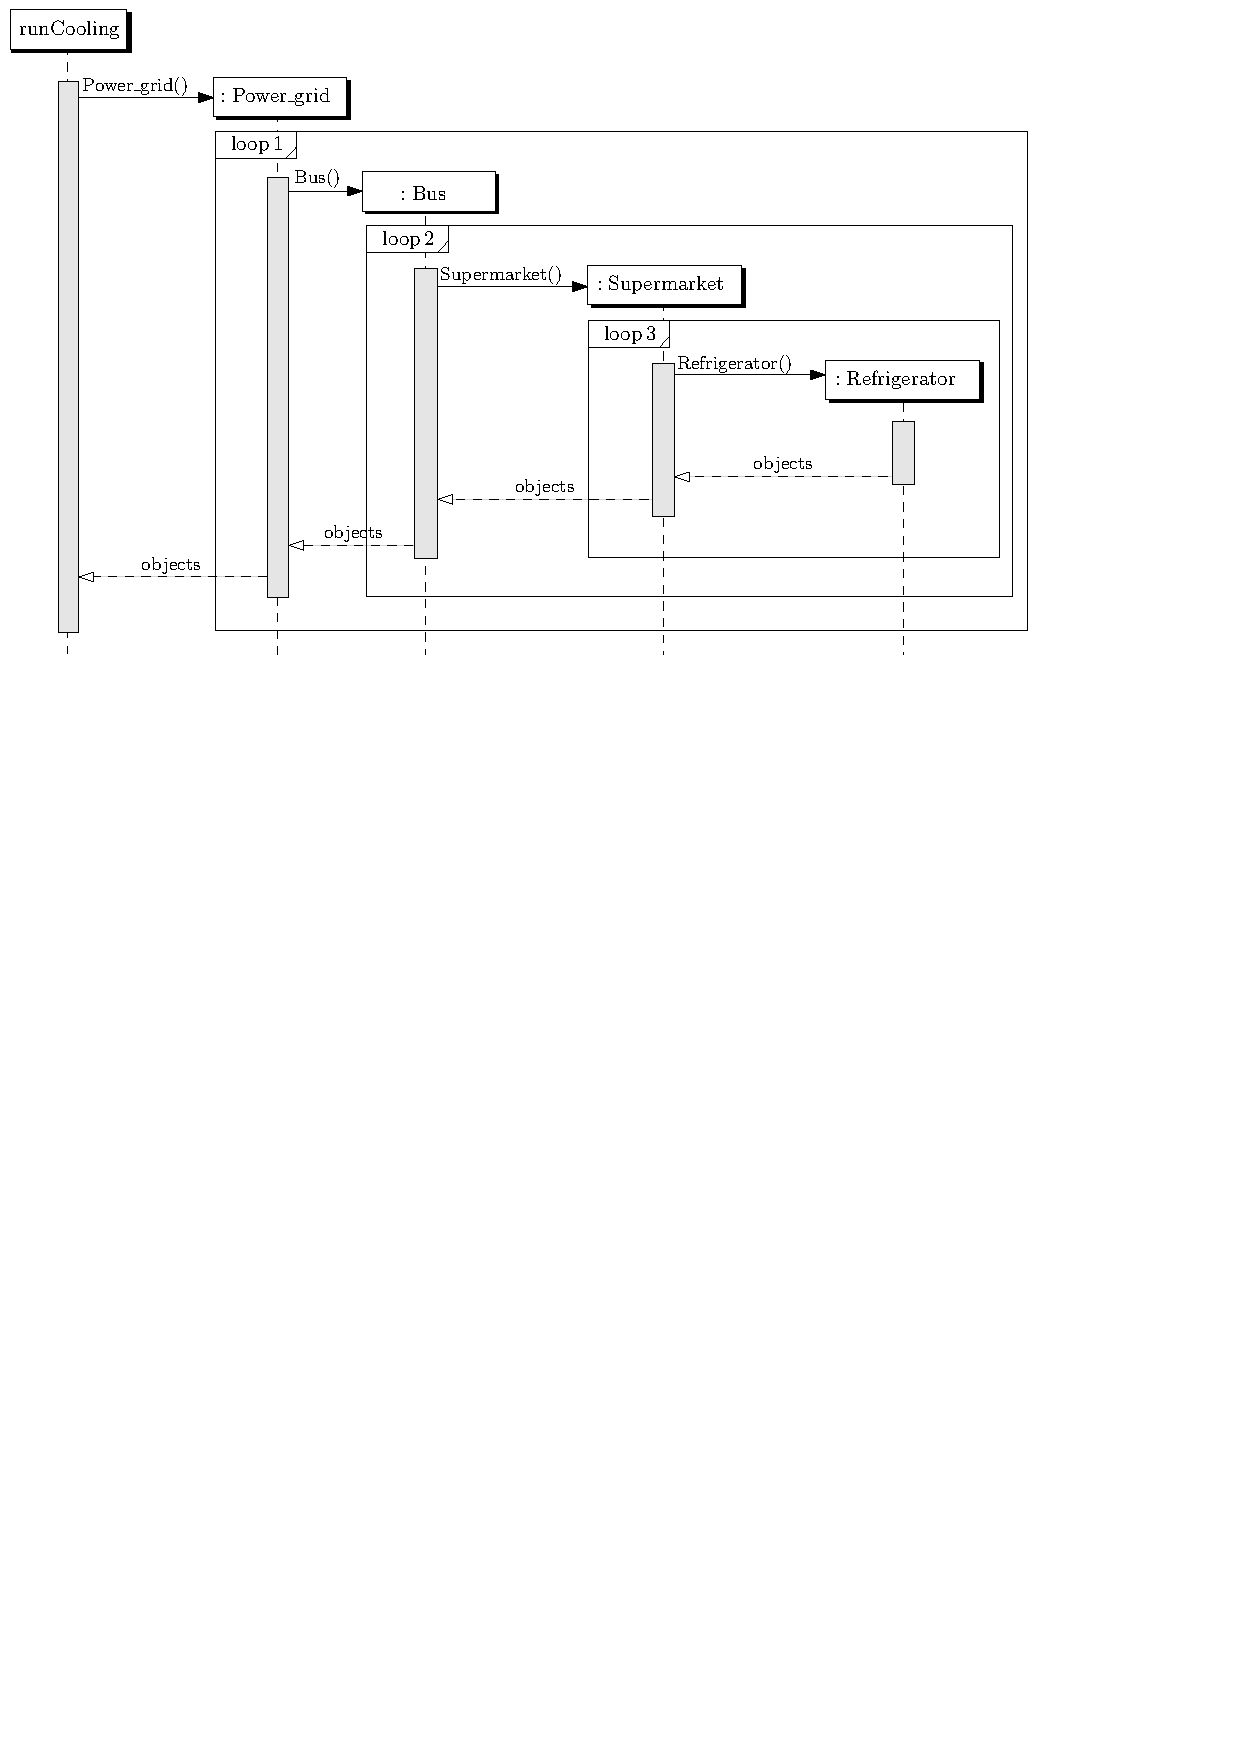
\includegraphics[scale=0.8]{images/Theorie_Super/sequence_one}
	\end{center}
\end{figure}

